\chapter{Results}
\label{ch:results}

Five experiments were run. Unless stated otherwise the target is climate change (kg~\co/kg),
modelled as $\log_{10}$, and all numbers are out-of-fold over 5 folds (seed 42).

\section{E1 -- Model comparison}
\label{sec:e1}

\begin{table}[ht]
\centering\small
\caption{Model comparison for climate change under the two validation schemes. Best ML values in bold; ``proxy'' is the practitioner baseline.}
\label{tab:e1}
\begin{tabular}{@{}lrrrrrr@{}}
\toprule
& \multicolumn{3}{c}{Random 5-fold CV} & \multicolumn{3}{c}{Leave-sub-group-out CV} \\
\cmidrule(lr){2-4}\cmidrule(l){5-7}
Method & $R^2_{\log}$ & ${<}2\times$ (\%) & Spearman & $R^2_{\log}$ & ${<}2\times$ (\%) & Spearman \\
\midrule
Global median & $-0.01$ & 44.0 & $-0.02$ & $-0.03$ & 42.2 & $-0.20$ \\
Sub-group median (proxy) & 0.62 & 77.4 & 0.82 & 0.33 & 54.2 & 0.58 \\
Ridge & 0.81 & 89.2 & 0.91 & 0.57 & 69.0 & 0.77 \\
Random Forest & 0.83 & 91.0 & 0.92 & 0.58 & 69.9 & 0.77 \\
\textbf{XGBoost} & \textbf{0.84} & \textbf{91.1} & \textbf{0.92} & \textbf{0.62} & \textbf{72.4} & \textbf{0.78} \\
kNN on E5 embedding & 0.71 & 82.7 & 0.84 & 0.25 & 56.3 & 0.48 \\
XGBoost + kNN feature & 0.83 & 90.7 & 0.92 & 0.56 & 69.7 & 0.74 \\
\bottomrule
\end{tabular}
\end{table}

\begin{figure}[ht]
\centering
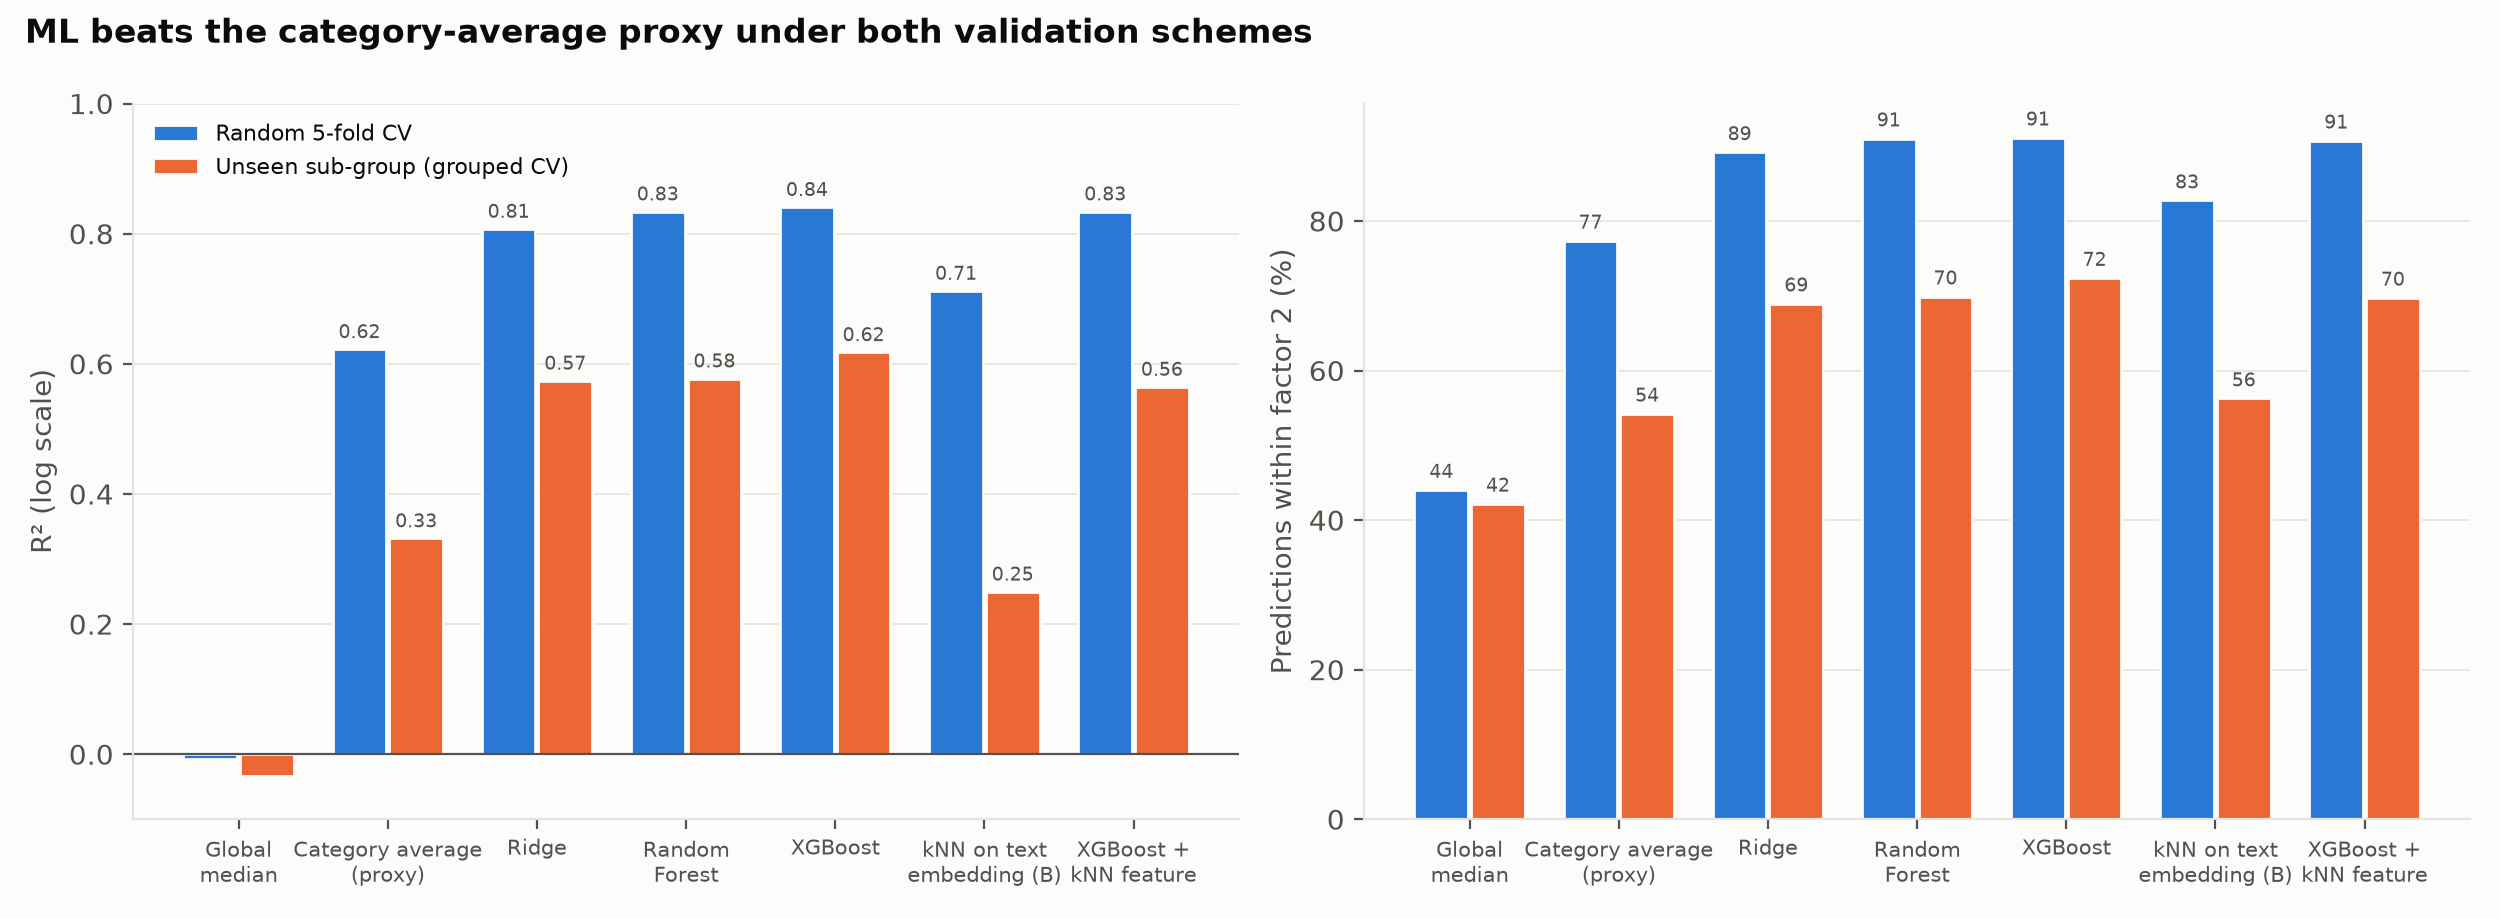
\includegraphics[width=\textwidth]{f3_model_comparison}
\caption{Model comparison: $R^2$ on the log scale (left) and share of predictions within a factor of two (right), for random and leave-sub-group-out CV.}
\label{fig:e1}
\end{figure}

Table~\ref{tab:e1} and Figure~\ref{fig:e1} answer \textbf{RQ1}. Under random CV, every ML model
clearly beats the category-average proxy; XGBoost raises $R^2_{\log}$ from 0.62 to 0.84 and the
within-factor-2 rate from 77\% to 91\%. Its median absolute percentage error is 19\% (proxy: 32\%)
and its MAE is 1.49~kg~\co/kg (proxy: 2.80). The Spearman correlation of 0.92 means that the
model ranks products almost correctly -- the property that matters most for screening.

The tree ensembles (Random Forest, XGBoost) outperform Ridge, indicating useful non-linear
interactions (e.g.\ the effect of ``chilled'' depends on the food group). XGBoost and Random
Forest are close; XGBoost is selected because it is best on the harder scheme.

\textbf{RQ2 -- generalisation.} When entire sub-groups are hidden, all methods degrade, as
expected. The proxy suffers most ($R^2$ 0.62 $\rightarrow$ 0.33): when a category is new, its
average is unknown and the method falls back to the group average. XGBoost retains $R^2=0.62$
and 72\% within a factor of two, because ingredient and name-word features transfer across
categories (e.g.\ \emph{beef} means high impact in any sub-group). The gap between the two schemes
(0.84 vs 0.62) is the honest measure of how much random CV benefits from near-duplicate products.

Figure~\ref{fig:pred} shows out-of-fold predictions against AGRIBALYSE values. Most points lie
within the factor-of-two band across four orders of magnitude. The largest errors are
instructive rather than random:
\begin{itemize}
  \item \textbf{Unique products} -- tap water (0.0003~kg~\co/kg) is predicted at 0.77 because
  nothing similar exists in the training data.
  \item \textbf{Air freight} -- mango pulp flown from Brazil (11.6, predicted 0.79) and French
  beans flown from Kenya (7.1, predicted 0.75). Only two products carry the air-freight flag, so
  the model cannot learn its effect; a rare but decisive life-cycle choice is invisible to a
  data-driven model.
  \item \textbf{High-impact tropical crops in low-impact groups} -- cocoa powder (29.1, predicted
  1.6), ground coffee (8.4, predicted 0.8) and cocoa butter sit in the beverage and fat groups,
  whose typical members have far lower footprints.
\end{itemize}
These failure modes point directly to the features a future version needs (transport mode,
origin, crop type), and they are discussed in Chapter~\ref{ch:discussion}.

\begin{figure}[ht]
\centering
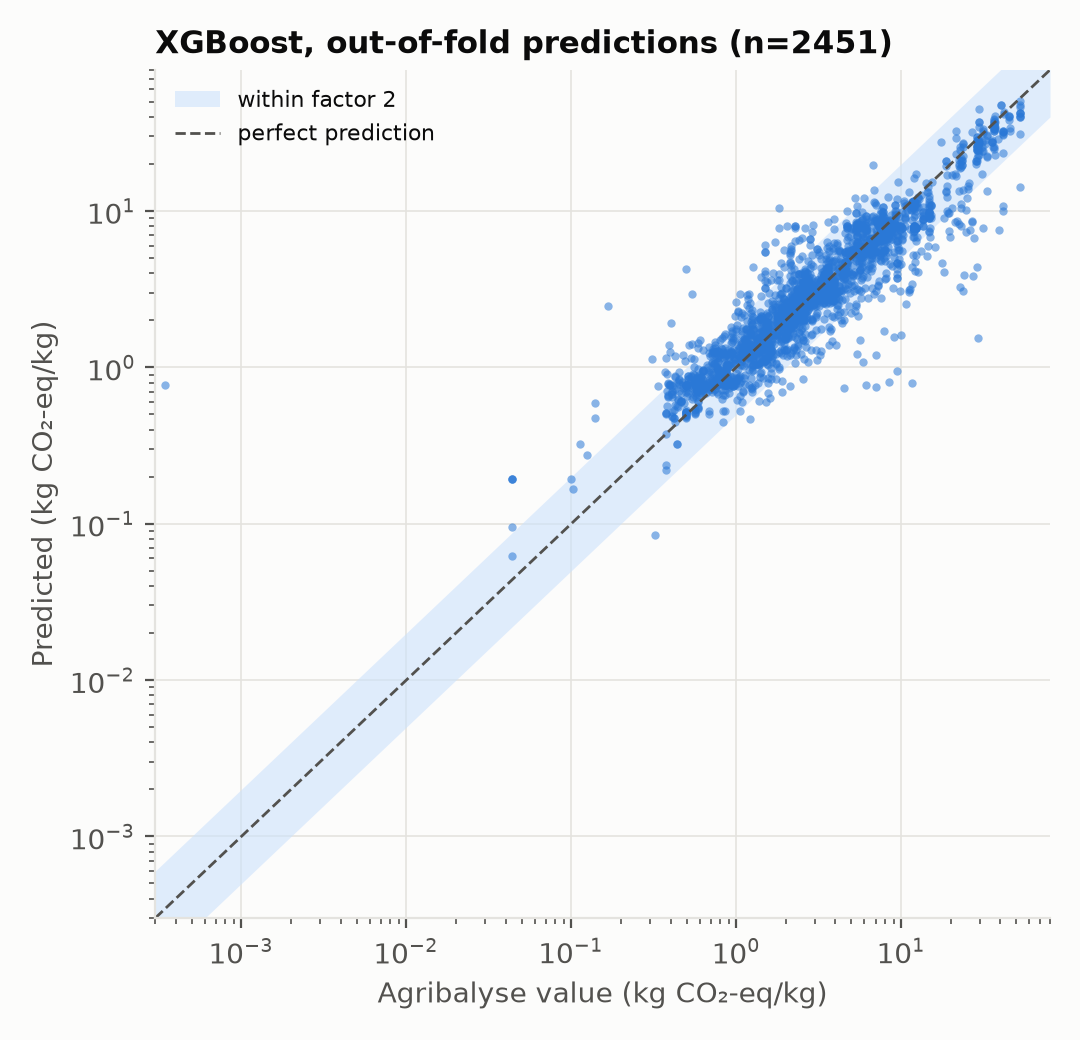
\includegraphics[width=0.62\textwidth]{f4_pred_vs_actual}
\caption{XGBoost out-of-fold predictions vs.\ AGRIBALYSE values (random CV, log--log). Shaded band: within a factor of two.}
\label{fig:pred}
\end{figure}

\section{E2 -- Feature ablation}
\label{sec:ablation}

\begin{table}[ht]
\centering\small
\caption{Feature ablation with XGBoost ($R^2_{\log}$ / within factor 2).}
\label{tab:e2}
\begin{tabular}{@{}lcc@{}}
\toprule
Feature set & Random CV & Leave-sub-group-out \\
\midrule
META (categories, storage, preparation, packaging) & 0.70 / 79.2\% & 0.48 / 64.0\% \\
+ ING (recipe ingredients) & 0.75 / 84.6\% & 0.52 / 67.2\% \\
+ TXT (product-name words) & \textbf{0.84 / 91.1\%} & \textbf{0.62 / 72.4\%} \\
+ KNN (E5-embedding neighbours) & 0.83 / 90.7\% & 0.56 / 69.7\% \\
\bottomrule
\end{tabular}
\end{table}

\begin{figure}[ht]
\centering
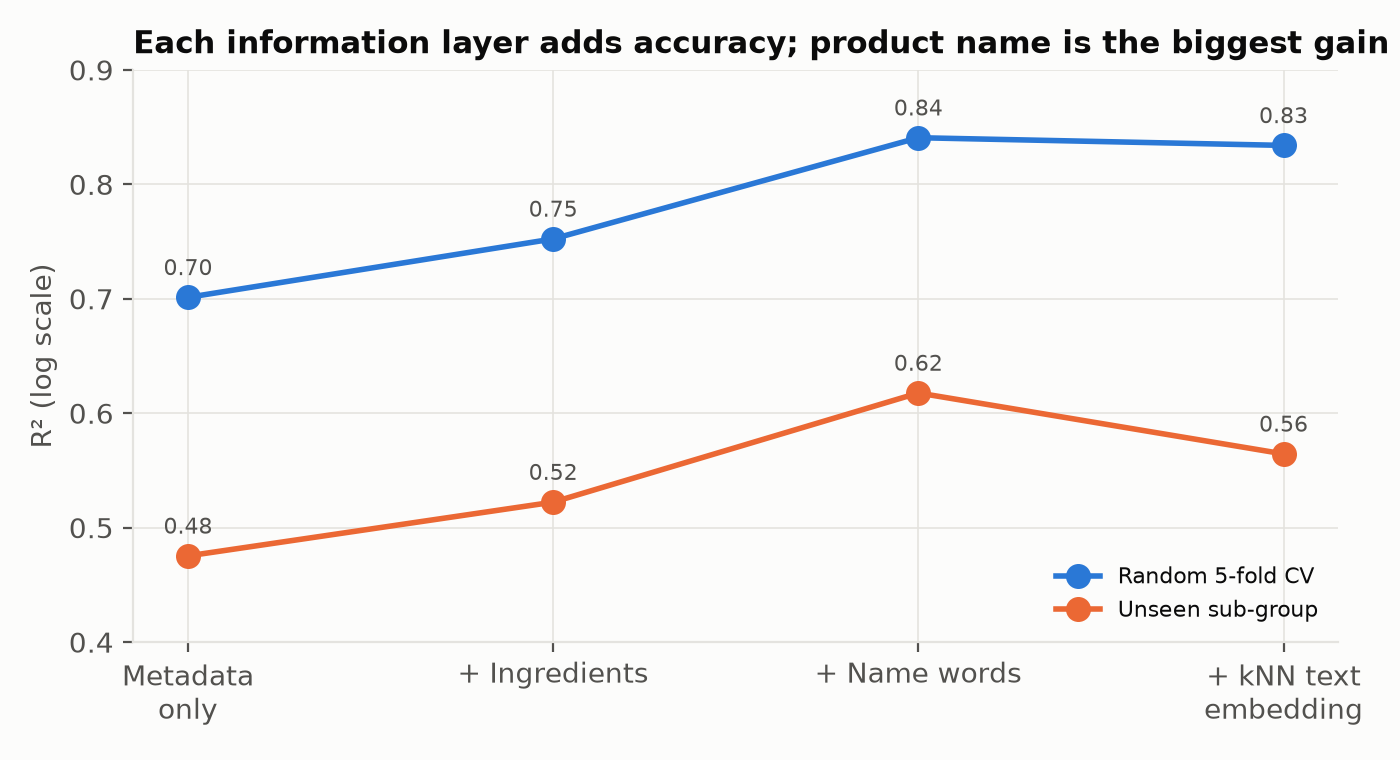
\includegraphics[width=0.8\textwidth]{f5_ablation}
\caption{Ablation: accuracy as information layers are added.}
\label{fig:ablation}
\end{figure}

Each pre-LCA information layer adds accuracy (Table~\ref{tab:e2}, Figure~\ref{fig:ablation}).
Metadata alone already beat the proxy (0.70 vs 0.62), ingredients add 0.05, and \textbf{product-name
words give the largest single gain} (+0.09 random, +0.10 unseen). This agrees with the stage
analysis in Chapter~\ref{ch:data}: impact is dominated by agriculture, i.e.\ by \emph{what} the
food is, which the name states directly (``lamb'', ``beef'', ``chocolate'').

A notable \emph{negative result} is that stacking the E5-embedding kNN estimate as a feature
did \emph{not} help; it slightly reduced accuracy, particularly on unseen sub-groups (0.62
$\rightarrow$ 0.56). The kNN estimate is largely redundant with the explicit word features, and on
new categories it imports the footprint of superficially similar but differently produced foods.
Embeddings were therefore kept for \emph{mapping} (Module B), where they excel (Section~\ref{sec:e5}),
and not used as a predictive feature.

\section{E3 -- Generalisation to other impact categories}
\label{sec:e3}

\begin{table}[ht]
\centering\small
\caption{Proxy vs.\ XGBoost for six EF 3.0 indicators (random CV).}
\label{tab:e3}
\begin{tabular}{@{}lrcccc@{}}
\toprule
& & \multicolumn{2}{c}{$R^2_{\log}$} & \multicolumn{2}{c}{Within $2\times$ (\%)} \\
\cmidrule(lr){3-4}\cmidrule(l){5-6}
Impact category (unit per kg) & $n$ & Proxy & XGBoost & Proxy & XGBoost \\
\midrule
Climate change (kg \co) & 2,451 & 0.62 & \textbf{0.84} & 77.4 & \textbf{91.1} \\
EF single score (mPt) & 2,451 & 0.64 & \textbf{0.84} & 78.2 & \textbf{90.4} \\
Land use (Pt) & 2,417 & 0.58 & \textbf{0.78} & 66.4 & \textbf{80.4} \\
Water use (m\textsuperscript{3} world-eq) & 2,450 & 0.27 & \textbf{0.64} & 64.8 & \textbf{80.5} \\
Marine eutrophication (kg N-eq) & 2,451 & 0.59 & \textbf{0.78} & 69.4 & \textbf{83.5} \\
Particulate matter (disease inc.) & 2,451 & 0.70 & \textbf{0.86} & 73.2 & \textbf{85.8} \\
\bottomrule
\end{tabular}
\end{table}

\begin{figure}[ht]
\centering
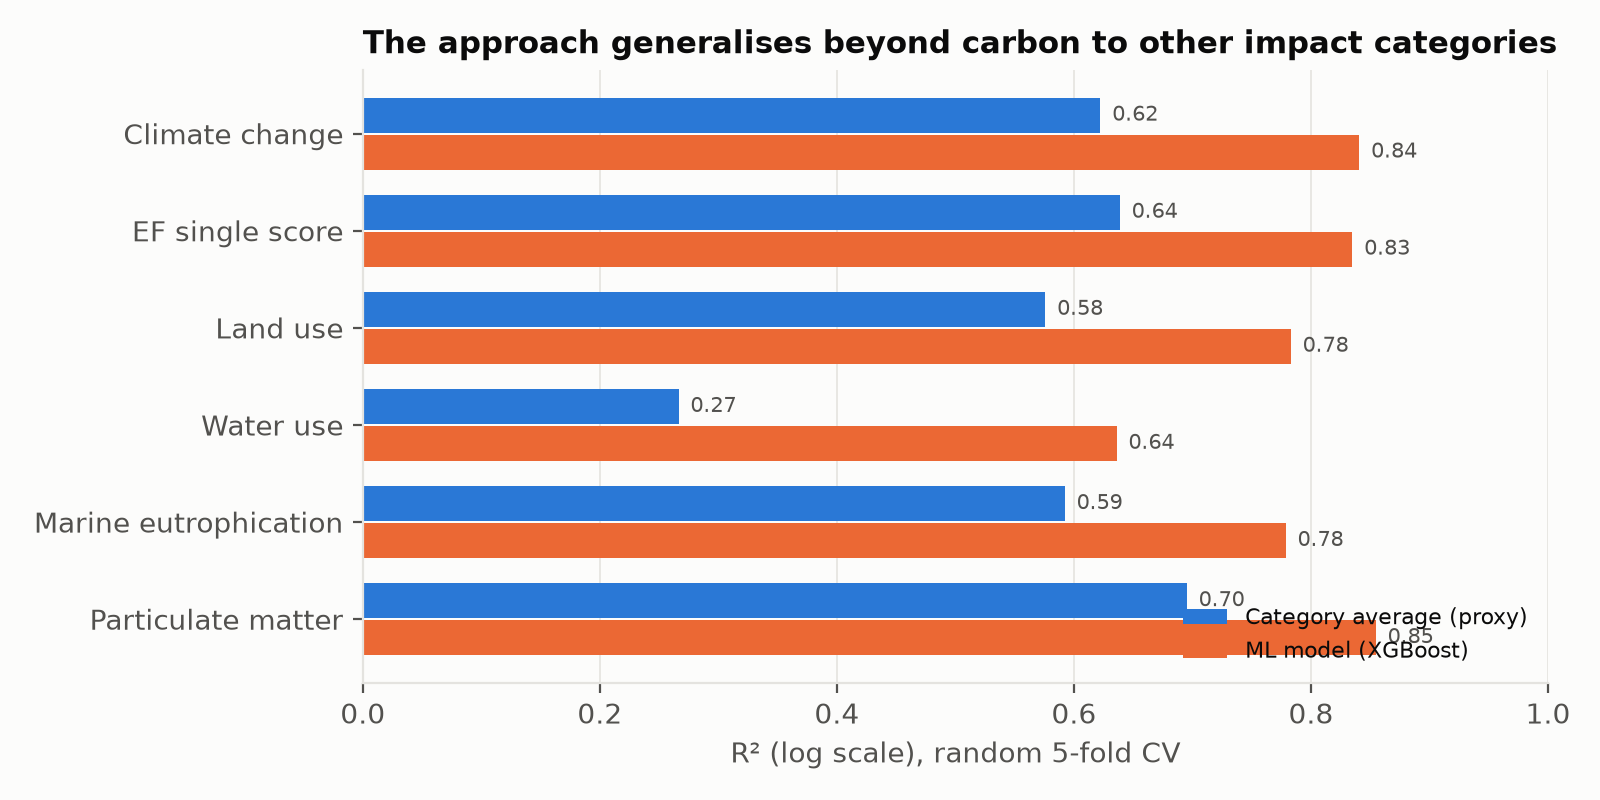
\includegraphics[width=0.85\textwidth]{f8_multi_impact}
\caption{The same pipeline, retrained per indicator, beats the proxy on all six impact categories.}
\label{fig:e3}
\end{figure}

The same pipeline, retrained per indicator without any change, improves on the proxy for every
category (Table~\ref{tab:e3}, Figure~\ref{fig:e3}). The largest relative gain is for \textbf{water
use} ($R^2$ 0.27 $\rightarrow$ 0.64): water scarcity depends strongly on crop and irrigation, which
category averages capture poorly but ingredient and name features capture well. Land use and
water remain the hardest indicators, consistent with their strong dependence on sourcing
location, which is not among the inputs.

\section{E4 -- Calibrated uncertainty}
\label{sec:e4}

\begin{table}[ht]
\centering\small
\caption{Mondrian conformal 90\% intervals (nested calibration).}
\label{tab:e4}
\begin{tabular}{@{}lcc@{}}
\toprule
Scheme & Empirical coverage & Median interval \\
\midrule
Random CV & 91.1\% & $\hat I\ \times\!/\!\div\ 2.0$ \\
Leave-sub-group-out CV & 87.2\% & $\hat I\ \times\!/\!\div\ 3.3$ \\
\bottomrule
\end{tabular}
\end{table}

\begin{figure}[ht]
\centering
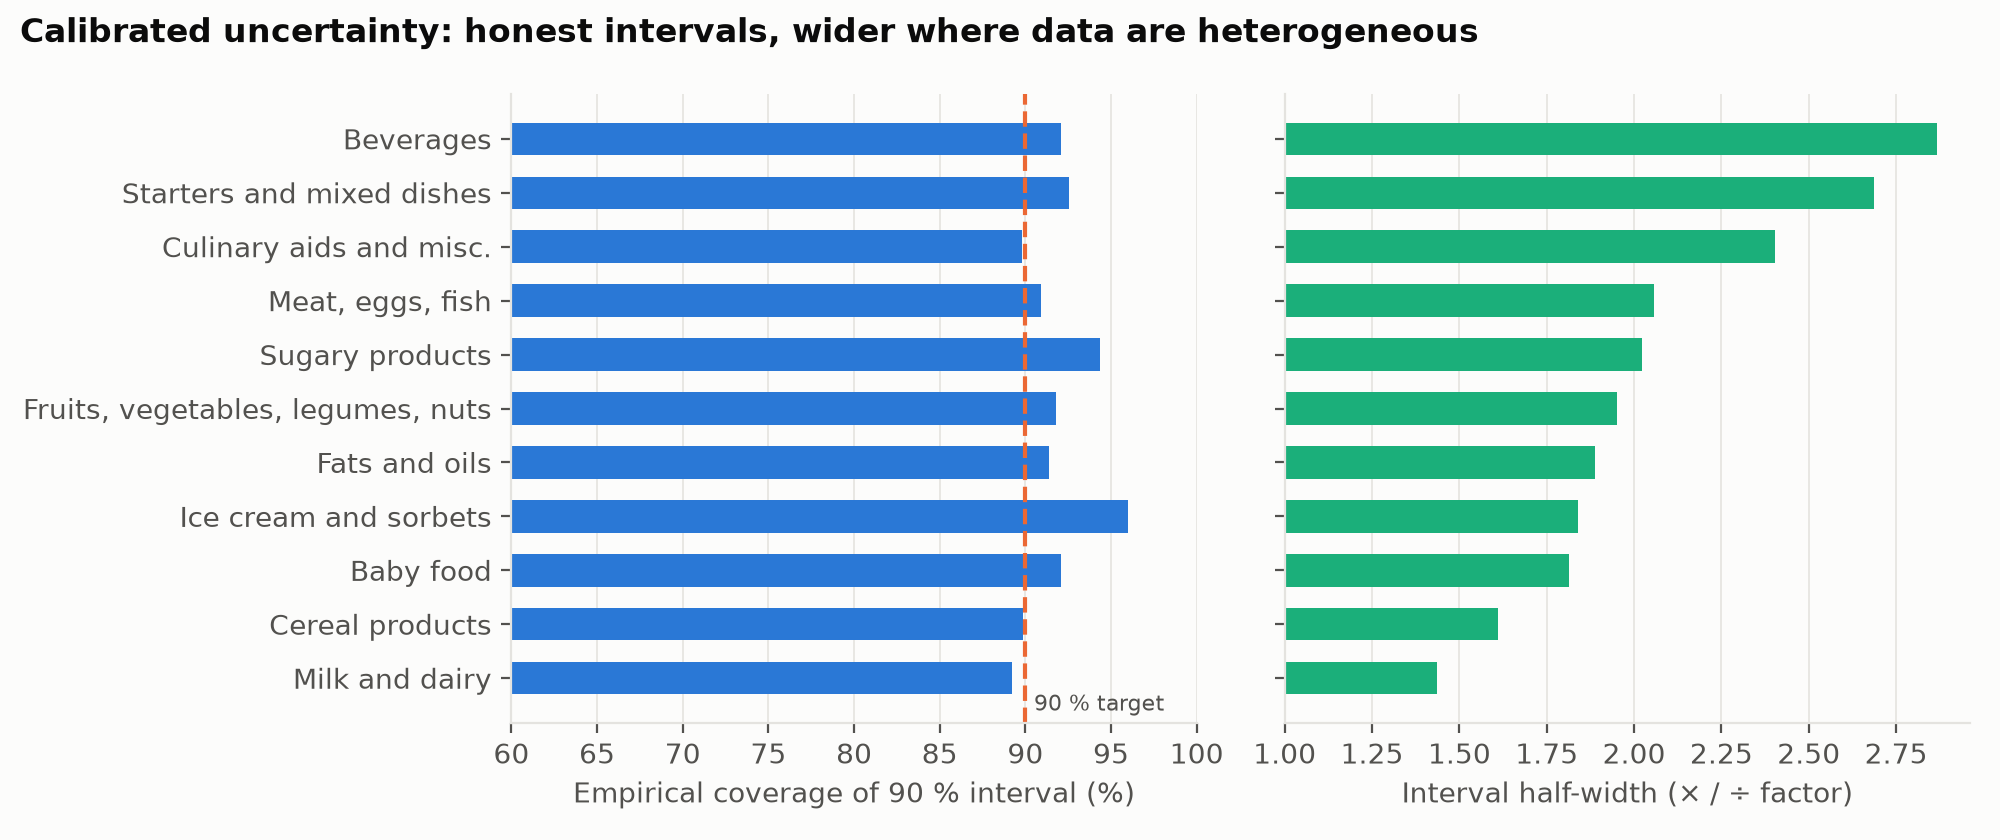
\includegraphics[width=\textwidth]{f10_conformal}
\caption{Per-group coverage (left) and interval half-width as a multiplicative factor (right), random CV.}
\label{fig:conformal}
\end{figure}

Under random CV the 90\% intervals achieve 91.1\% coverage, i.e.\ they are \emph{calibrated}
(Table~\ref{tab:e4}). Coverage is close to the target in every food group (89--96\%,
Figure~\ref{fig:conformal}), while widths adapt to difficulty: dairy products get
$\times\!/\!\div\,1.4$, mixed dishes $\times\!/\!\div\,2.7$ and beverages $\times\!/\!\div\,2.9$.
This is the practical value of the Mondrian variant.

On unseen sub-groups, overall coverage drops slightly to 87.2\% and intervals widen to
$\times\!/\!\div\,3.3$. The aggregate hides an instructive failure: coverage falls to 46\% for
\emph{milk and dairy}, 71\% for \emph{culinary aids} and 72\% for \emph{sugary products}. Dairy
sub-groups differ systematically (e.g.\ cheeses are several times more impactful than milks per
kg), and the calibration residuals, drawn from the remaining dairy sub-groups, are too small for
a new one. This is exactly the exchangeability assumption of conformal prediction being violated
under distribution shift, and it is reported here because it defines where the tool's intervals
should not be trusted: genuinely new product types within otherwise homogeneous groups.

\section{E5 -- Mapping descriptions to LCA datasets (Module B)}
\label{sec:e5}

\begin{table}[ht]
\centering\small
\caption{Mapping benchmark (2,451 queries per task). ``Borrow ${<}2\times$'': share of top-1 matches whose footprint is within a factor of two of the true product.}
\label{tab:e5}
\begin{tabular}{@{}lcccccc@{}}
\toprule
& \multicolumn{3}{c}{T1: French name $\rightarrow$ English DB} & \multicolumn{3}{c}{T2: 3-word query $\rightarrow$ full name} \\
\cmidrule(lr){2-4}\cmidrule(l){5-7}
Encoder & Top-1 & Top-5 & Borrow${<}2\times$ & Top-1 & Top-5 & Borrow${<}2\times$ \\
\midrule
TF-IDF char n-gram & 27.7 & 48.3 & 63.4 & 69.4 & 92.2 & 93.8 \\
MiniLM-L12 multilingual & 28.4 & 43.0 & 64.7 & 64.7 & 87.0 & 93.5 \\
LaBSE & \textbf{59.7} & \textbf{76.8} & \textbf{84.0} & 62.2 & 79.2 & 89.3 \\
E5-base multilingual & 48.2 & 67.5 & 78.3 & 74.0 & 94.6 & \textbf{97.1} \\
\textbf{E5-small (chosen)} & 47.1 & 66.0 & 78.8 & \textbf{75.0} & \textbf{94.9} & 96.8 \\
Hybrid TF-IDF + E5-small & 34.8 & 58.2 & 68.7 & 71.5 & 93.2 & 94.8 \\
\bottomrule
\end{tabular}
\end{table}

\begin{figure}[ht]
\centering
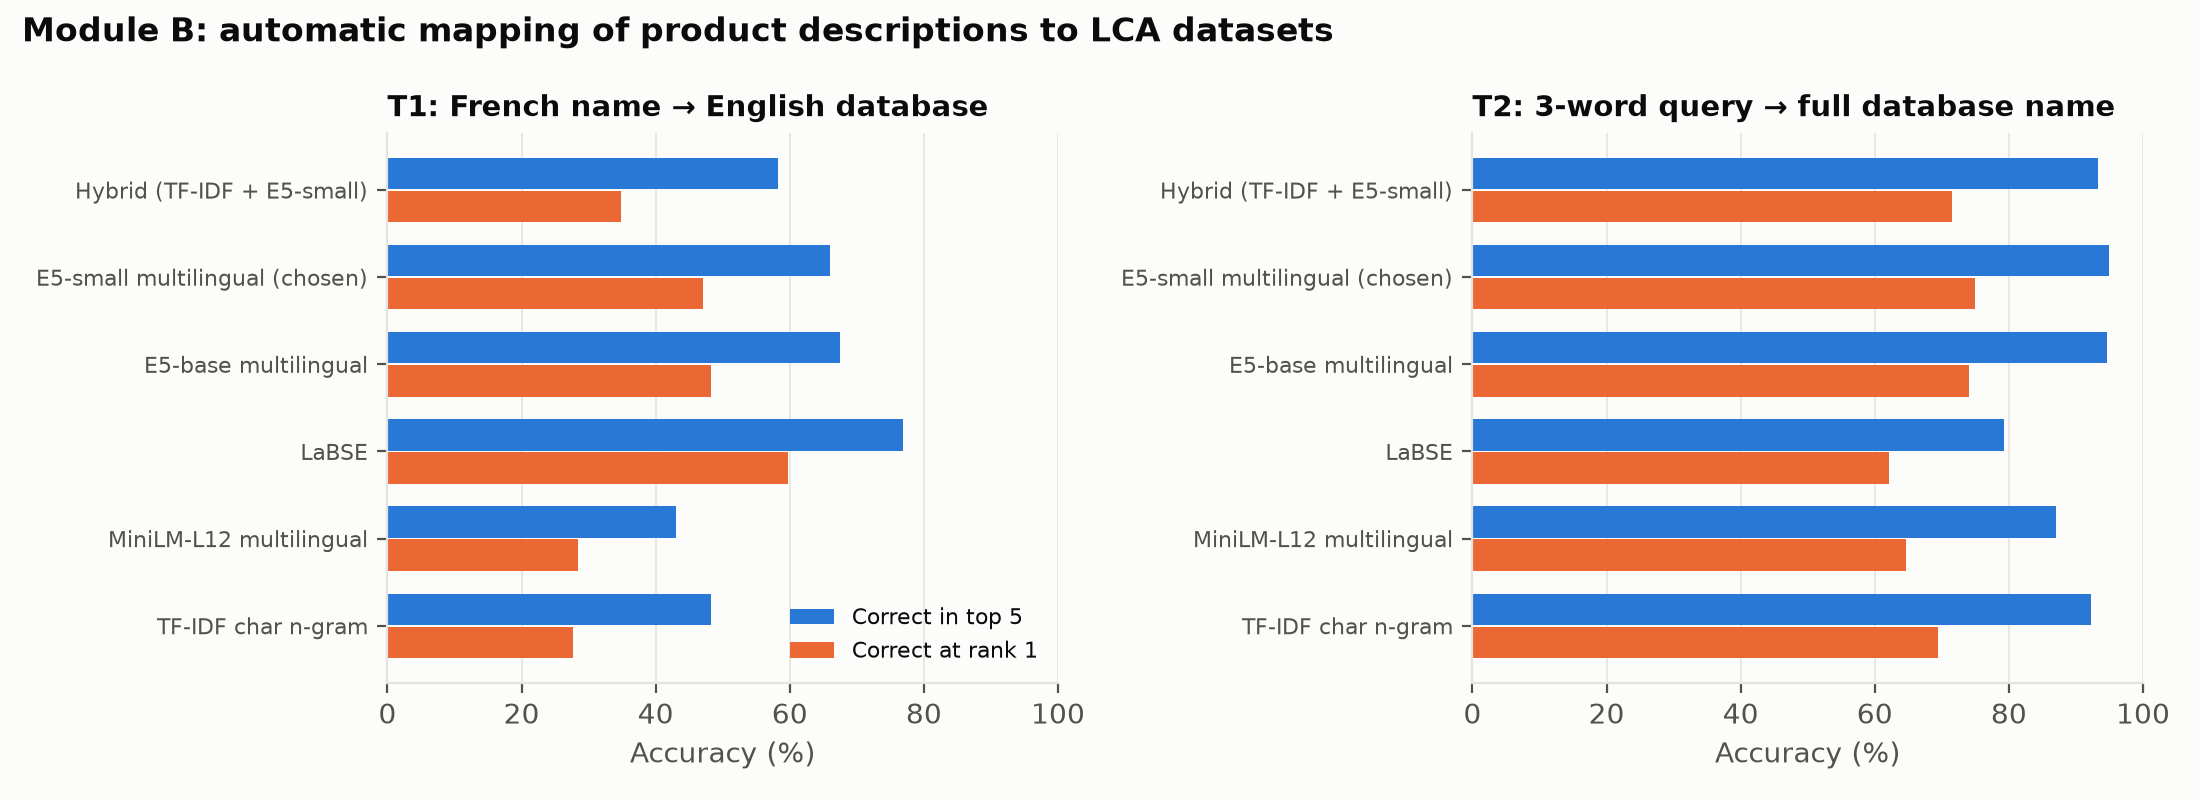
\includegraphics[width=\textwidth]{f9_matching}
\caption{Top-1 and top-5 mapping accuracy for both tasks.}
\label{fig:e5}
\end{figure}

Table~\ref{tab:e5} and Figure~\ref{fig:e5} answer \textbf{RQ4}. On the realistic terse-query task,
E5-small retrieves the exact dataset at rank 1 for 75\% of queries and within the top five for
95\%; borrowing the top-1 footprint lands within a factor of two of the truth for 97\% of queries.
Because the correctness criterion is strict (exact name), many ``errors'' are near-duplicates
(raw vs.\ cooked, fresh vs.\ frozen): 96\% of top-1 matches fall in the correct sub-group.

Three findings shaped the design:
\begin{itemize}
  \item \textbf{Encoder choice matters more than expected.} The widely used MiniLM model is no
  better than lexical TF-IDF across languages (28\% top-1), while E5 and LaBSE are far better.
  \item \textbf{No single best encoder.} LaBSE, trained for translation pairs, is best cross-lingually
  (60\% top-1) but worst on terse queries; E5-small is best on terse queries and second-best
  cross-lingually while being about four times smaller than E5-base. E5-small was chosen because
  terse queries are the primary use case.
  \item \textbf{Naive hybrids can hurt.} Averaging TF-IDF and E5 scores \emph{reduced} accuracy,
  because the two similarity scales have very different ranges; E5 alone is used.
\end{itemize}

\section{Explainability (SHAP)}
\label{sec:shap}

\begin{figure}[ht]
\centering
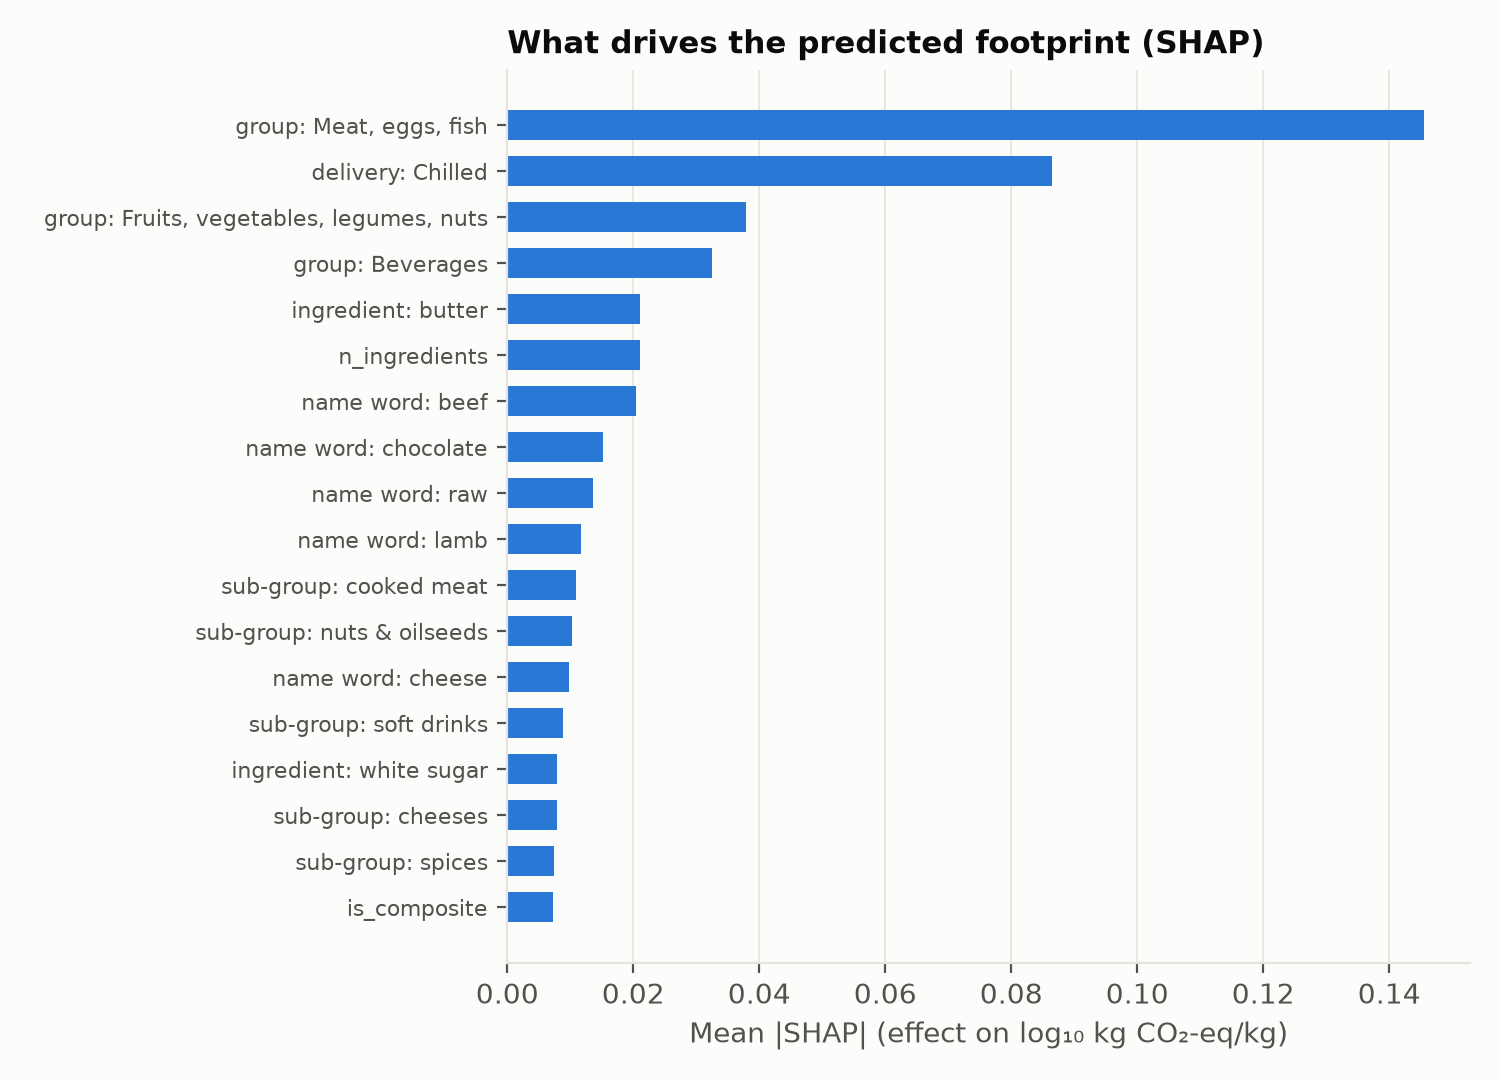
\includegraphics[width=0.85\textwidth]{f6_shap_importance}
\caption{Global feature importance: mean absolute SHAP value on the $\log_{10}$ scale.}
\label{fig:shap}
\end{figure}

\begin{figure}[ht]
\centering
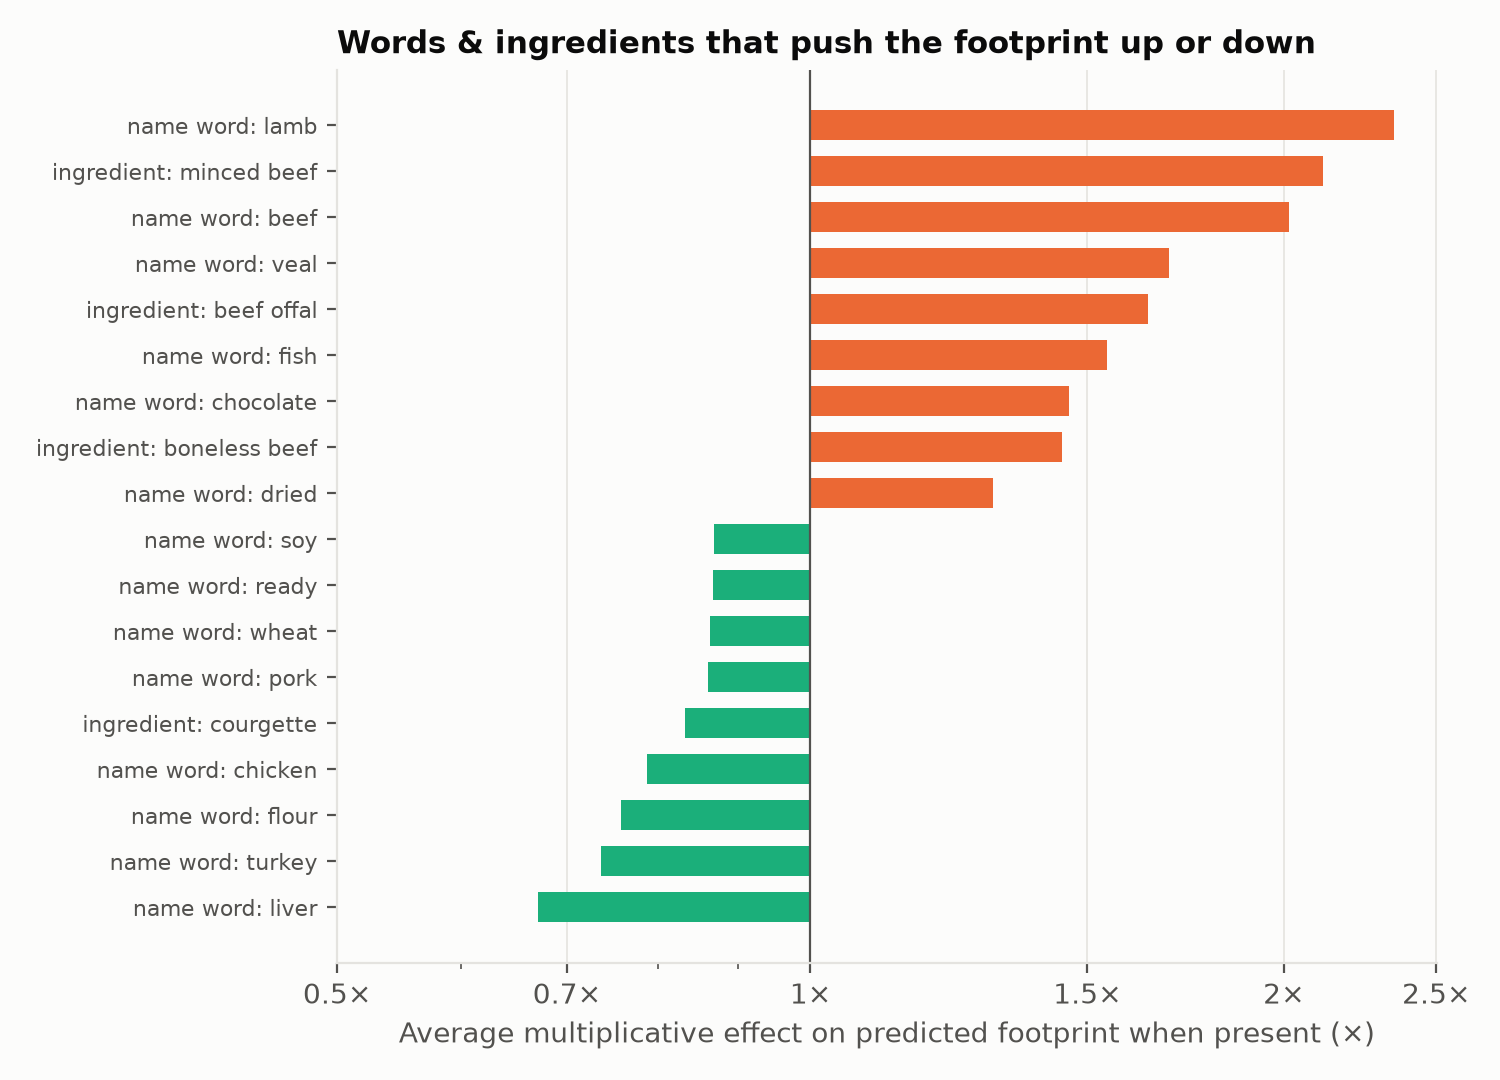
\includegraphics[width=0.85\textwidth]{f7_shap_direction}
\caption{Average multiplicative effect of name words and ingredients when present (orange: raises, green: lowers the estimate).}
\label{fig:shapdir}
\end{figure}

Figures~\ref{fig:shap} and~\ref{fig:shapdir} answer \textbf{RQ3}. Globally, the most influential
features are membership of the meat/eggs/fish group, chilled delivery, the fruit-and-vegetable and
beverage groups, butter as an ingredient, recipe size and the words \emph{beef}, \emph{chocolate}
and \emph{lamb}. Directionally (Figure~\ref{fig:shapdir}), \emph{lamb} multiplies the estimate by
about 2.4, minced beef by 2.1, \emph{beef} by 2.0 and \emph{veal} by 1.7, whereas \emph{chicken},
\emph{turkey} and \emph{pork} lower it relative to other meats. This ordering -- ruminant meat
$>$ pork $>$ poultry -- reproduces the well-established hierarchy in the food-LCA literature
\citep{poore2018}, and the large effect of \emph{chocolate} reflects the high land-use-change
emissions of cocoa. The model has therefore learned domain-consistent patterns rather than
spurious ones.

One important caveat for interpretation: \emph{chilled delivery} ranks second, but this does not
mean refrigeration causes high impacts. Chilled products are predominantly fresh meat, fish and
dairy, so ``chilled'' acts as a \emph{proxy} for animal products. SHAP explains the \emph{model},
not the physical system; causal statements require LCA modelling, not feature attributions.

\section{Summary of findings}

\begin{table}[ht]
\centering\small
\caption{Answers to the research questions.}
\begin{tabularx}{\textwidth}{@{}lX@{}}
\toprule
RQ & Finding \\
\midrule
RQ1 & XGBoost on pre-LCA features: $R^2_{\log}=0.84$, 91\% within $2\times$, Spearman 0.92 vs proxy 0.62 / 77\% / 0.82; consistent gains across six impact categories. \\
RQ2 & On unseen sub-groups $R^2_{\log}=0.62$ (proxy 0.33). 90\% conformal intervals are calibrated in-distribution (91.1\%) and slightly under-cover on new categories (87.2\%), with failures concentrated in dairy. \\
RQ3 & SHAP recovers the ruminant $>$ pork $>$ poultry hierarchy and the cocoa effect; ``chilled'' is a correlate of animal products, not a cause. \\
RQ4 & E5-small: 95\% top-5 on terse queries, 66\% top-5 cross-lingual; encoder choice is critical and no single encoder wins both tasks. \\
\bottomrule
\end{tabularx}
\end{table}
